\chapter{AVX2 grayscale, line by line}\label{ch:gray}

Reminder: $Y=(77R+150G+29B+128)\gg8$. The scalar code does this for one pixel per loop iteration. The AVX2 code converts \textbf{16 pixels per iteration}.

\section{Problem 1: the three channels are interleaved}

Memory contains \code{R0 G0 B0 R1 G1 B1 R2 \dots}. To multiply all red values by 77 with one instruction we need 16 reds next to each other in a register, and likewise for green and blue. Getting from the interleaved layout to three separate registers is called \emph{deinterleaving}.

Sixteen pixels are 48 bytes: exactly three 16-byte loads. Call them $v_0$ (bytes 0--15), $v_1$ (bytes 16--31) and $v_2$ (bytes 32--47).

\begin{center}
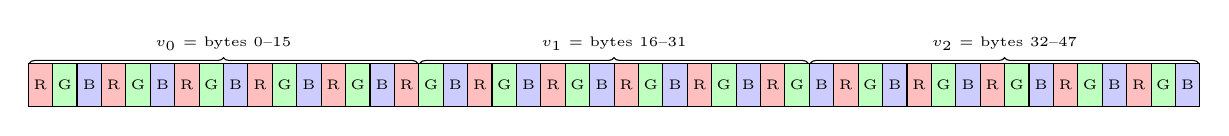
\begin{tikzpicture}[x=0.31cm,y=0.7cm,font=\tiny]
\foreach \i in {0,...,47} {
  \pgfmathtruncatemacro{\c}{mod(\i,3)}
  \pgfmathtruncatemacro{\p}{int(\i/3)}
  \node[draw,minimum width=0.31cm,minimum height=0.55cm,inner sep=0,
        fill=\ifcase\c red!25\or green!25\else blue!20\fi] at (\i,0) {\ifcase\c R\or G\or B\fi};
}
\foreach \k in {0,1,2} {
  \draw[decorate,decoration={brace,amplitude=2pt}] (16*\k-0.45,0.4) -- node[above=1pt]{$v_{\k}$ = bytes \the\numexpr16*\k\relax--\the\numexpr16*\k+15\relax} (16*\k+15.45,0.4);
}
\end{tikzpicture}
\end{center}

The reds are at byte positions $0,3,6,\dots,45$: six of them in $v_0$, five in $v_1$, five in $v_2$. \code{pshufb} (\code{\_mm\_shuffle\_epi8}) takes a register of data and a register of \emph{indices}: output byte $i$ is the data byte whose number is given in the index byte $i$; an index with its top bit set (we use \code{0x80}) produces a zero byte. So for each colour we build three index vectors, one per source register, which collect that colour's bytes into their final positions and leave zeros elsewhere. OR-ing the three partial results gives all 16 values of that colour in order.

\begin{center}
\small
\begin{tabular}{@{}cccc@{}}\toprule
 & mask for $v_0$ & mask for $v_1$ & mask for $v_2$\\ \midrule
\textbf{R} & \texttt{ 0  3  6  9 12 15 -- -- -- -- -- -- -- -- -- --} & \texttt{-- -- -- -- -- --  2  5  8 11 14 -- -- -- -- --} & \texttt{-- -- -- -- -- -- -- -- -- -- --  1  4  7 10 13} \\
\textbf{G} & \texttt{ 1  4  7 10 13 -- -- -- -- -- -- -- -- -- -- --} & \texttt{-- -- -- -- --  0  3  6  9 12 15 -- -- -- -- --} & \texttt{-- -- -- -- -- -- -- -- -- -- --  2  5  8 11 14} \\
\textbf{B} & \texttt{ 2  5  8 11 14 -- -- -- -- -- -- -- -- -- -- --} & \texttt{-- -- -- -- --  1  4  7 10 13 -- -- -- -- -- --} & \texttt{-- -- -- -- -- -- -- -- -- --  0  3  6  9 12 15} \\
\bottomrule\end{tabular}

{\footnotesize output byte $i$ = input byte at the listed index; \texttt{--} means index \texttt{0x80} (write 0)}
\end{center}

The tables are built by the compiler at compile time from one formula: pixel $i$'s colour-$c$ byte sits at global position $g=3i+c$, so it is read from source register $\lfloor g/16\rfloor$ at index $g\bmod16$.

\lstinputlisting{snippets/code_avx2_masks.cpp}

\section{Problem 2: the arithmetic must not overflow}

After deinterleaving, each colour is 16 bytes. We widen them to 16-bit lanes (\code{cvtepu8\_epi16}), multiply by 77, 150, 29 (\code{mullo\_epi16}, keeps the low 16 bits of each product) and add (with the $+128$). We showed in Chapter~\ref{ch:math} that the largest value is $65\,408<65\,536$: no wrap-around, so the low 16 bits of the products are the full products and plain 16-bit adds are exact. The shift \code{srli\_epi16(\dots,8)} divides by 256; it is a \emph{logical} shift, which is right because the values are unsigned.

\section{Problem 3: narrowing back to bytes}

The 16 results are 16-bit values in $[0,255]$ in one 256-bit register. \code{packus\_epi16} of the low and high 128-bit halves produces one 16-byte register in the original order, which is stored with one \code{storeu}.

\section{The complete kernel}

\lstinputlisting{snippets/code_avx2_gray.cpp}

\begin{plain}
\textbf{The tail.} The loop condition \code{x + 16 <= w} guarantees that the three loads (which read bytes $3x\dots3x+47$) stay inside the row: row $y$ has $3w$ bytes and the last pixel read is $x+15\le w-1$. The remaining 0--15 pixels use the scalar formula. Because the test suite uses \emph{tight} images (stride equal to the row size and an allocation that ends exactly after the last row), AddressSanitizer would flag a load one byte too far.
\end{plain}

\section{Why this is only a few times faster, not 16 times}

Per 16 pixels the code issues 3 loads, 9 shuffles, 6 ORs, 3 widenings, 3 multiplies, 4 adds, 1 shift, 1 pack and 1 store: about 30 instructions, around 2 per pixel, compared with about 10 per pixel for scalar code. The speedup is therefore roughly 5$\times$ in the instruction count, and then memory starts to limit: the kernel reads 3 bytes and writes 1 byte per pixel and has very little arithmetic to hide the memory traffic. Chapter~\ref{ch:cache} puts a number on how close it gets to the memory ceiling.

\begin{sound}
``For gray I deinterleave 16 pixels with nine \code{pshufb} shuffles using constexpr index tables, widen to 16-bit, do the three multiplies and the rounding add in 16-bit lanes (the maximum is 65{,}408, so no overflow), shift, and pack back. I verified it against all 16.7 million RGB colours. It is a memory-heavy kernel, so I compared its throughput with a memory-copy yardstick.''
\end{sound}
